\documentclass[DM,authoryear,toc]{lsstdoc}
% lsstdoc documentation: https://lsst-texmf.lsst.io/lsstdoc.html
\input{meta}

% Package imports go here.

% Local commands go here.

%If you want glossaries
%\input{aglossary.tex}
%\makeglossaries

\title{Periodicity Analysis in Alert Production}

% Optional subtitle
% \setDocSubtitle{A subtitle}

\author{%
Anastasios Tzanidakis
}

\setDocRef{DMTN-221}
\setDocUpstreamLocation{\url{https://github.com/lsst-dm/dmtn-221}}

\date{\vcsDate}

% Optional: name of the document's curator
% \setDocCurator{The Curator of this Document}

\setDocAbstract{%
The baselined timeseries features to be computed in Alert Production include a Lomb-Scargle periodogram.  We assess the computational and scientific performance of several configurations on simulated alert data.
}


% Change history defined here.
% Order: oldest first.
% Fields: VERSION, DATE, DESCRIPTION, OWNER NAME.
% See LPM-51 for version number policy.
\setDocChangeRecord{%
  \addtohist{1}{YYYY-MM-DD}{Unreleased.}{Anastasios Tzanidakis, Eric Bellm}
}


\begin{document}

% Create the title page.
\maketitle
% Frequently for a technote we do not want a title page  uncomment this to remove the title page and changelog.
% use \mkshorttitle to remove the extra pages

% ADD CONTENT HERE
% You can also use the \input command to include several content files.

\section{Motivation}
The characterization of periodicity from time-series is a fundamental constraint to numerous astrophysical applications. Phenomenologically, estimating the periodicity and its significance can shed light on stellar pulsation theory \citep{Antonello:Antonello81}, distance estimation and mapping of the Galaxy through Cepeheids, Miras and RR Lyrae \citep{Skowron:Skowron2019}, constraint fundamental parameters of stellar binaries \citep{Farinella:Farinella1979}, and stellar rotation \citep{Walkowicz:Walkowicz13}. In the recent decade, the use of periodicity has also been extensively used as a feature to classify transient phenomena \citep{Richards:R13}.



\section{Synthetic Light Curves}
In this study we use the training set Extended LSST Astronomical Time-series Classification Challenge (ELAsTiCC) light curves. In short, ELAsTiCC is an end-to-end real-time pipeline for generating mock photometric alerts at the expected Legacy Survey of Time and Space (LSST) rate. The photometric alerts will be distributed in real-time to brokers to benchmark classification algorithms. The ELAsTiCC uses the V.1.7 cadence strategy from op_sims. A single detection is based on the DIA performance from DC2. Each light curve include photometric noise using Poisson noise that includes the equivalent area, background noise per unit area, sky and CCD read noise. Most importantly to this study, the training set light curves simulates forced photometry which we recommend the time series features to be calculated upon. Here we present two classes of periodic sources: RR Lyrae and eclipsing binaries. Both RRL's and EB's represent both the extrema of simple and complex periodic sources that will throughly test the underlying ability of the periodogram to find the correct period. Previous studies, such as work from \citep{Oluseyi:Oluseyi2012} have demonstrated the injection-recovery test for RR Lyrae. A detailed Jupyter notebook interacting and fetching the ELAsTiCC light curves can be found here. 

\begin{figure*}
  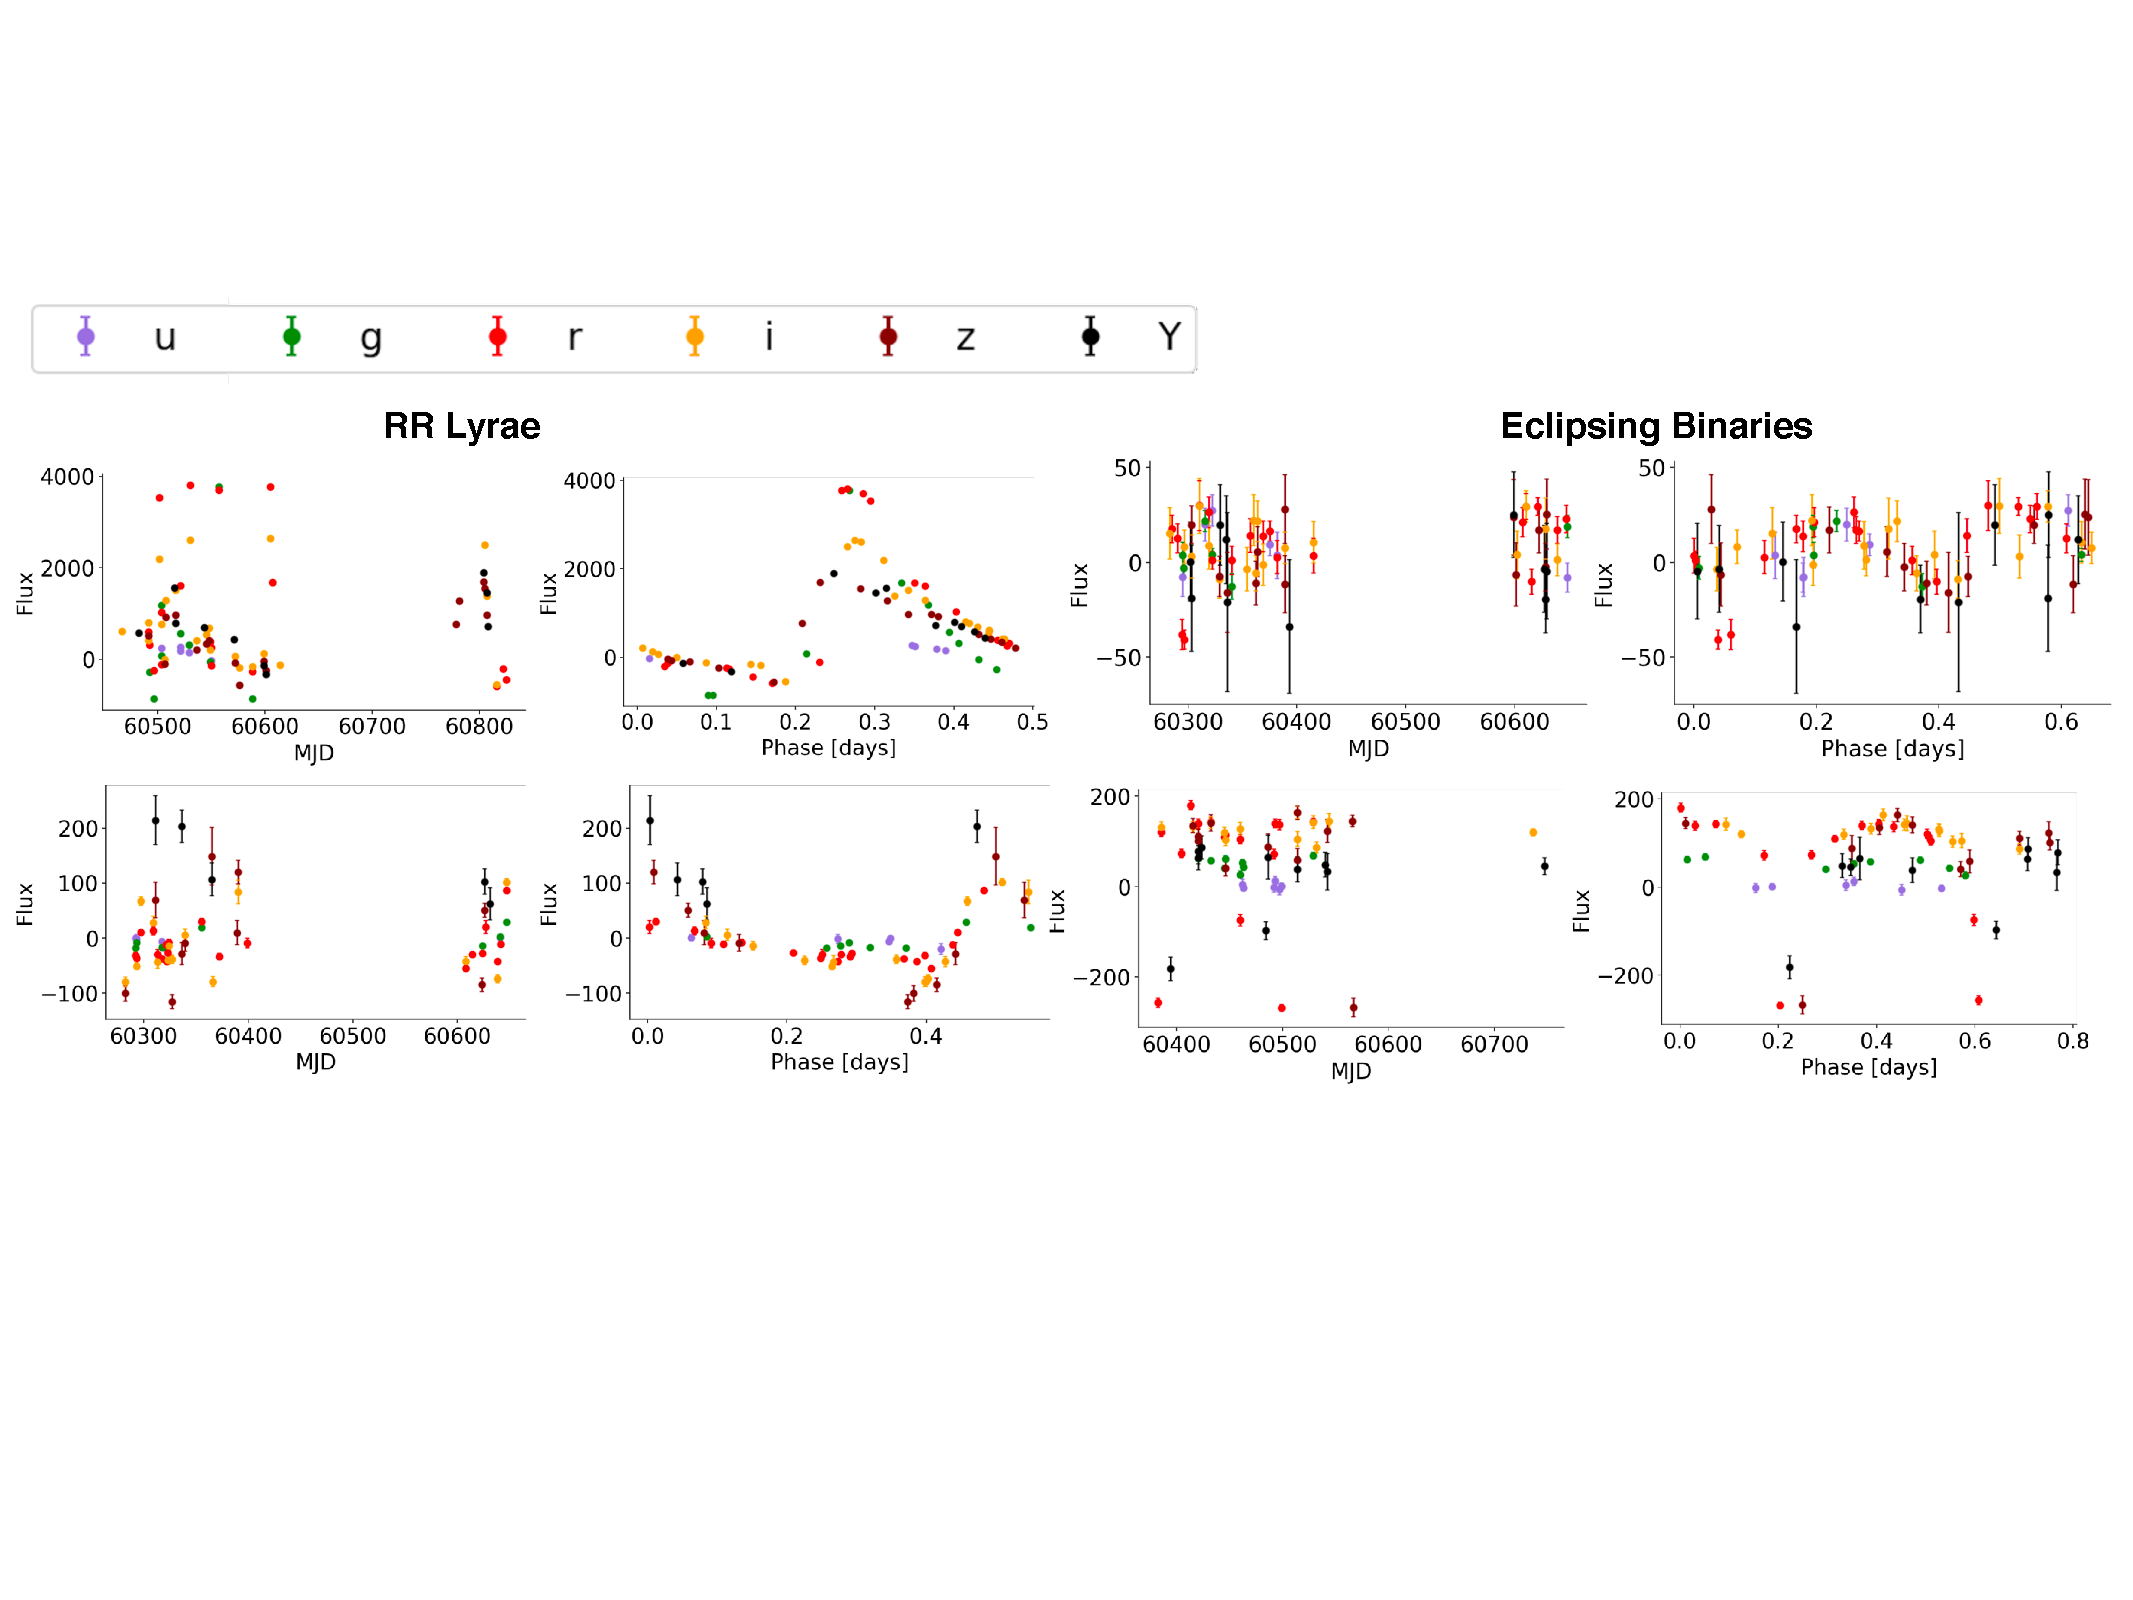
\includegraphics[width=0.9\textwidth]{figures/lightcurve_demo.pdf}
  \centering 
  \caption{The above panels demonstrate the multi-band light curves simulated from ElasTiCC using RR lyrae (left panel) and eclipsing binaries (right panel). The first column of each panel shows the observed light curves, and the second the phase folded light curves at the correct period after 12 months.}
  \label{fig:comp}
\end{figure*}


\section{Injection-Recovery Testing}
We consider two models of periodic phenomena: RR lyrae and eclipsing binaries ranging from a periods of 0.2 days to 10 days. All computations of the floating-mean Lomb-Scargle periodogram are using the out-of-box open-source Python package `gatspy` \citet{VanderPlas:VP2015}. 



\subsection{Single Band Lomb-Scargle Periodogram}

% TODO
\begin{itemize}
\item Injected vs recovered period plots eclipsing binaries and RRL
\item Fraction of correctly recovered periods using single-band Lomb-Scargle (for N=1...3 Fourier components)  
\end{itemize}

\begin{figure*}
  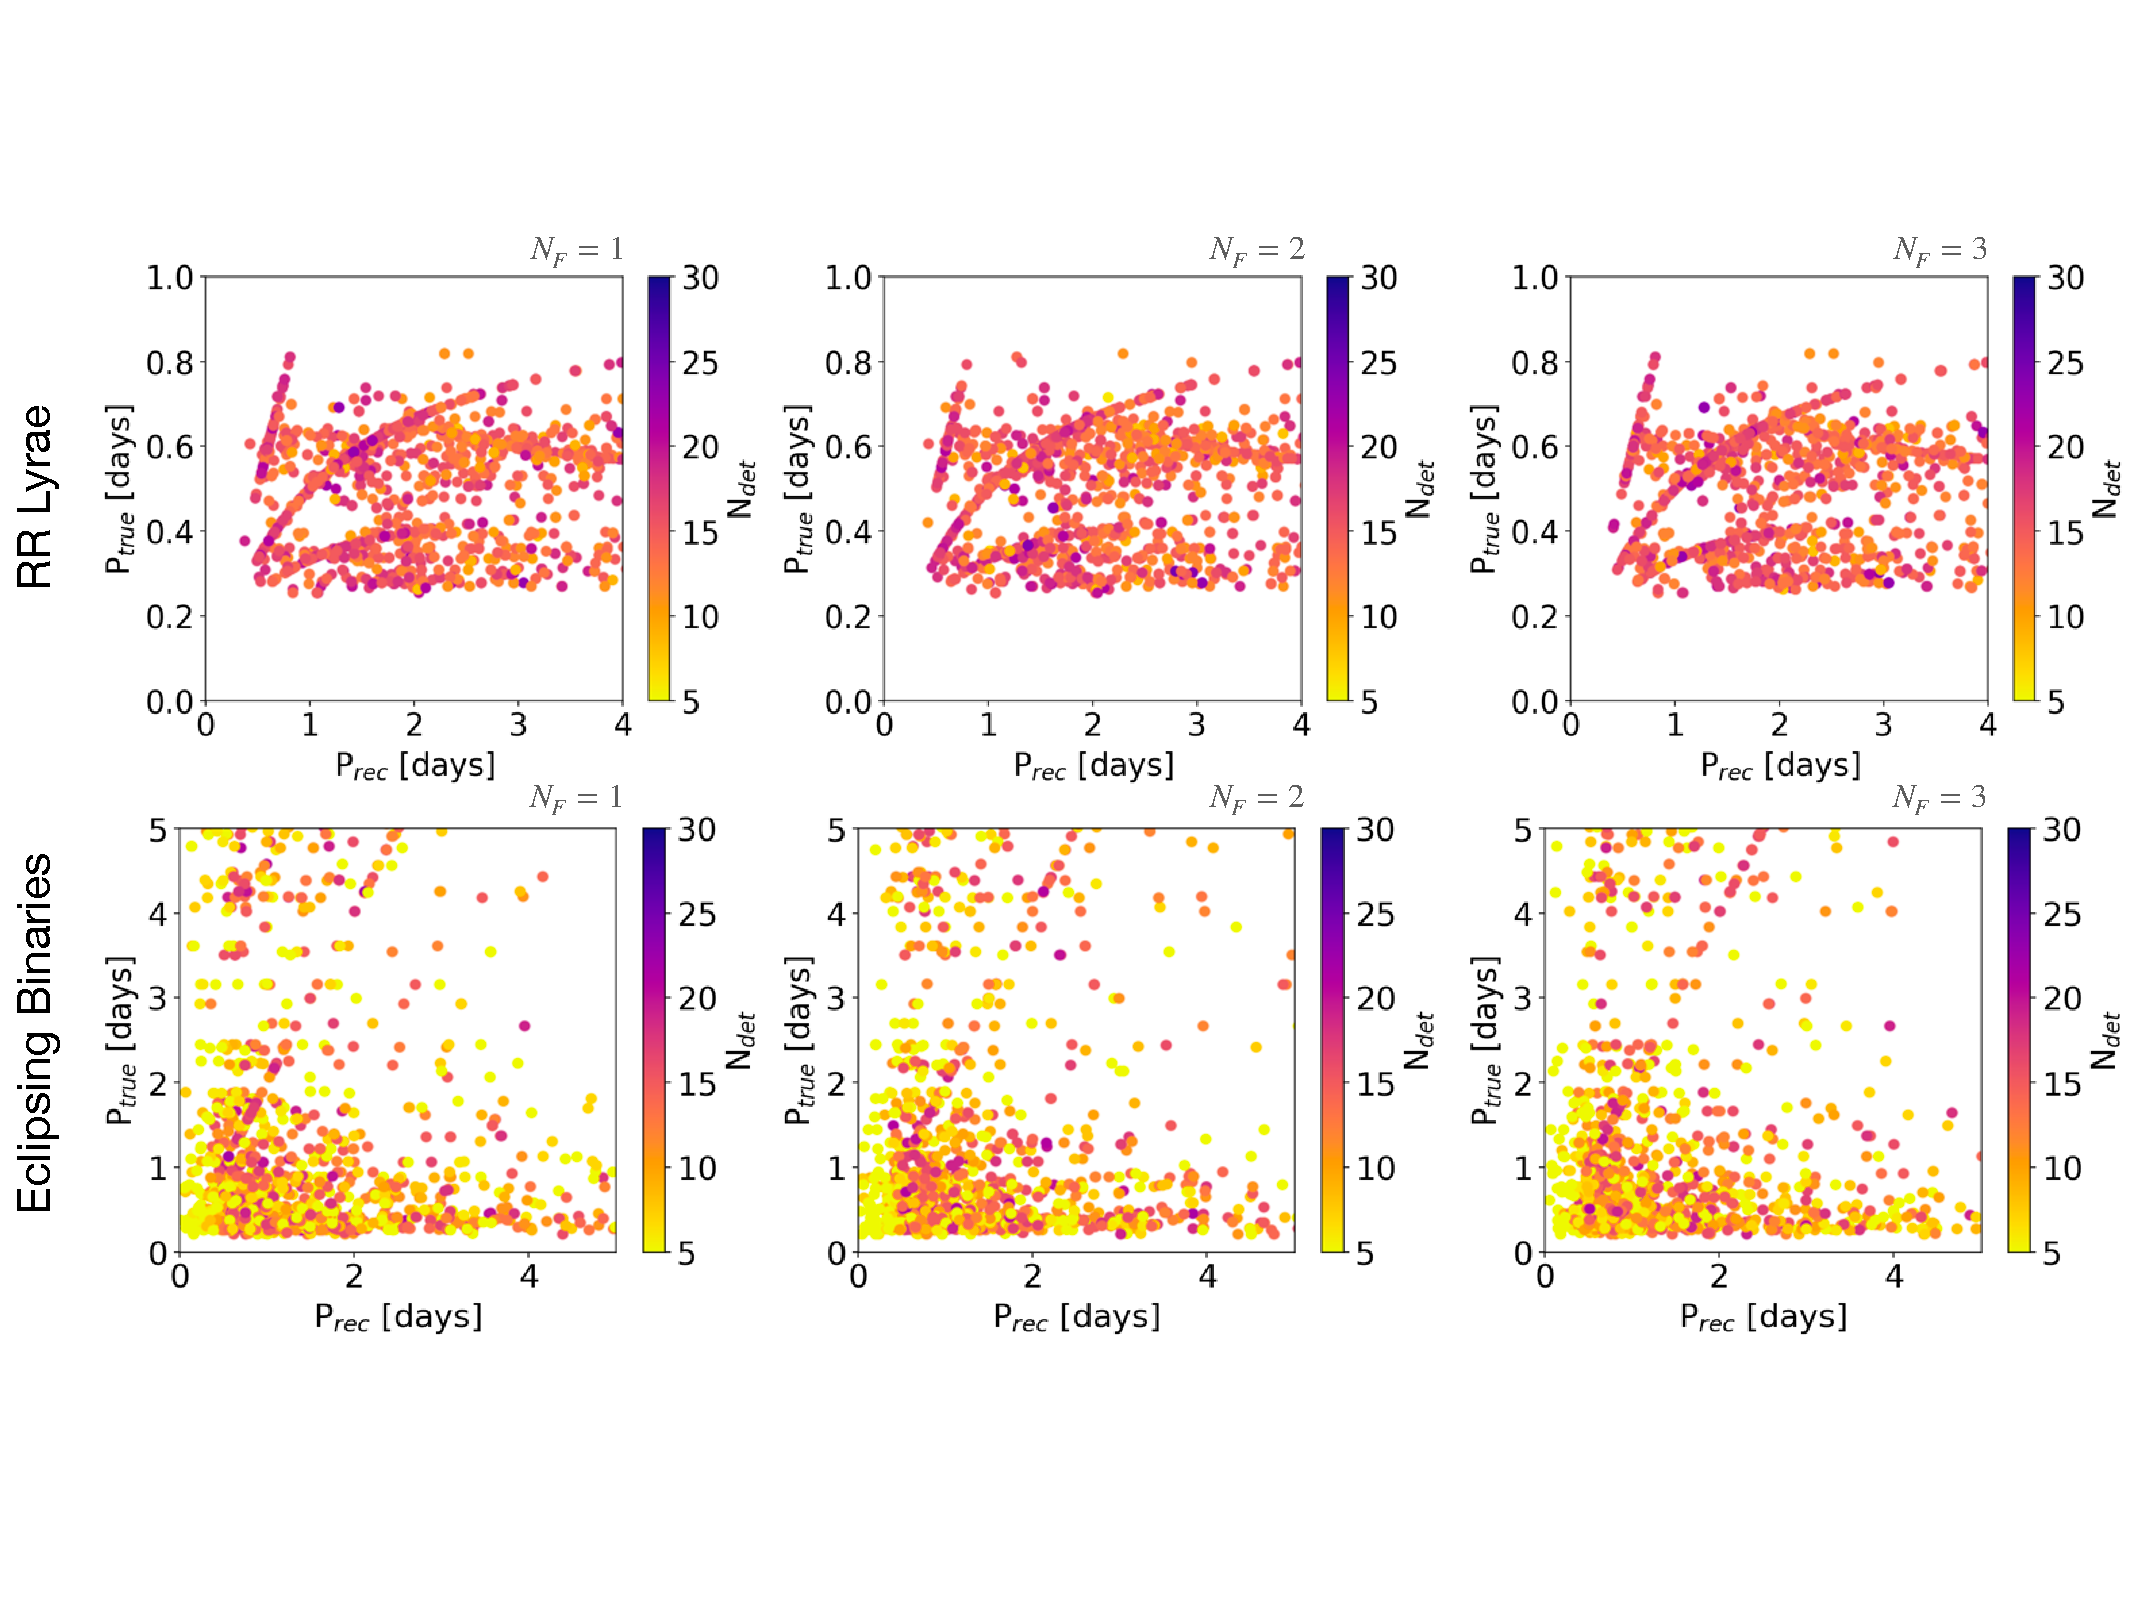
\includegraphics[width=0.9\textwidth]{figures/singleband_lsp.pdf}
  \centering 
  \caption{We show the injected (true period) versus recovered highest peak in the periodogram for a sample of 1000 RR lyrae and eclipsing binaries. Each column shows the period recovery for N=1 to N=3 Fourier components when computing the Lomb-Scargle periodogram.}
  \label{fig:comp}
\end{figure*}

However, given that only roughly 17 percent of each bandpass filter will be available, the single-band Lomb-Scargle misses by a higher margin the underlying true period. We now turn our attention to the multi-band Lomb-Scargle.

\subsection{Multi-Band Lomb-Scargle Periodogram}

Next, we test the multi-band Lomb-Scargle periodogram implementation adapted on `gatspy` to our ELAsTiCC light curves:
\begin{equation}
y_k(t \mid \omega, \theta)=& \theta_0+\sum_{n=1}^{M_{\text {base }}}\left[\theta_{2 n-1} \sin (n \omega t)+\theta_{2 n} \cos (n \omega t)\right] \\ & \theta_0^{(k)}+\sum_{n=1}^{M_{\text {band }}}\left[\theta_{2 n-1}^{(k)} \sin (n \omega t)+\theta_{2 n}^{(k)} \cos (n \omega t)\right] 
\end{equation}

% TODO
\begin{itemize}
\item Motivation and mathematical explanation of multi-band Lomb Scargle 
\item Injected vs recovered period plots eclipsing binaries and RRL
\item Fraction of correctly recovered periods using single-band Lomb-Scargle (for N=1...3 Fourier components)  
\end{itemize}


\begin{figure*}
  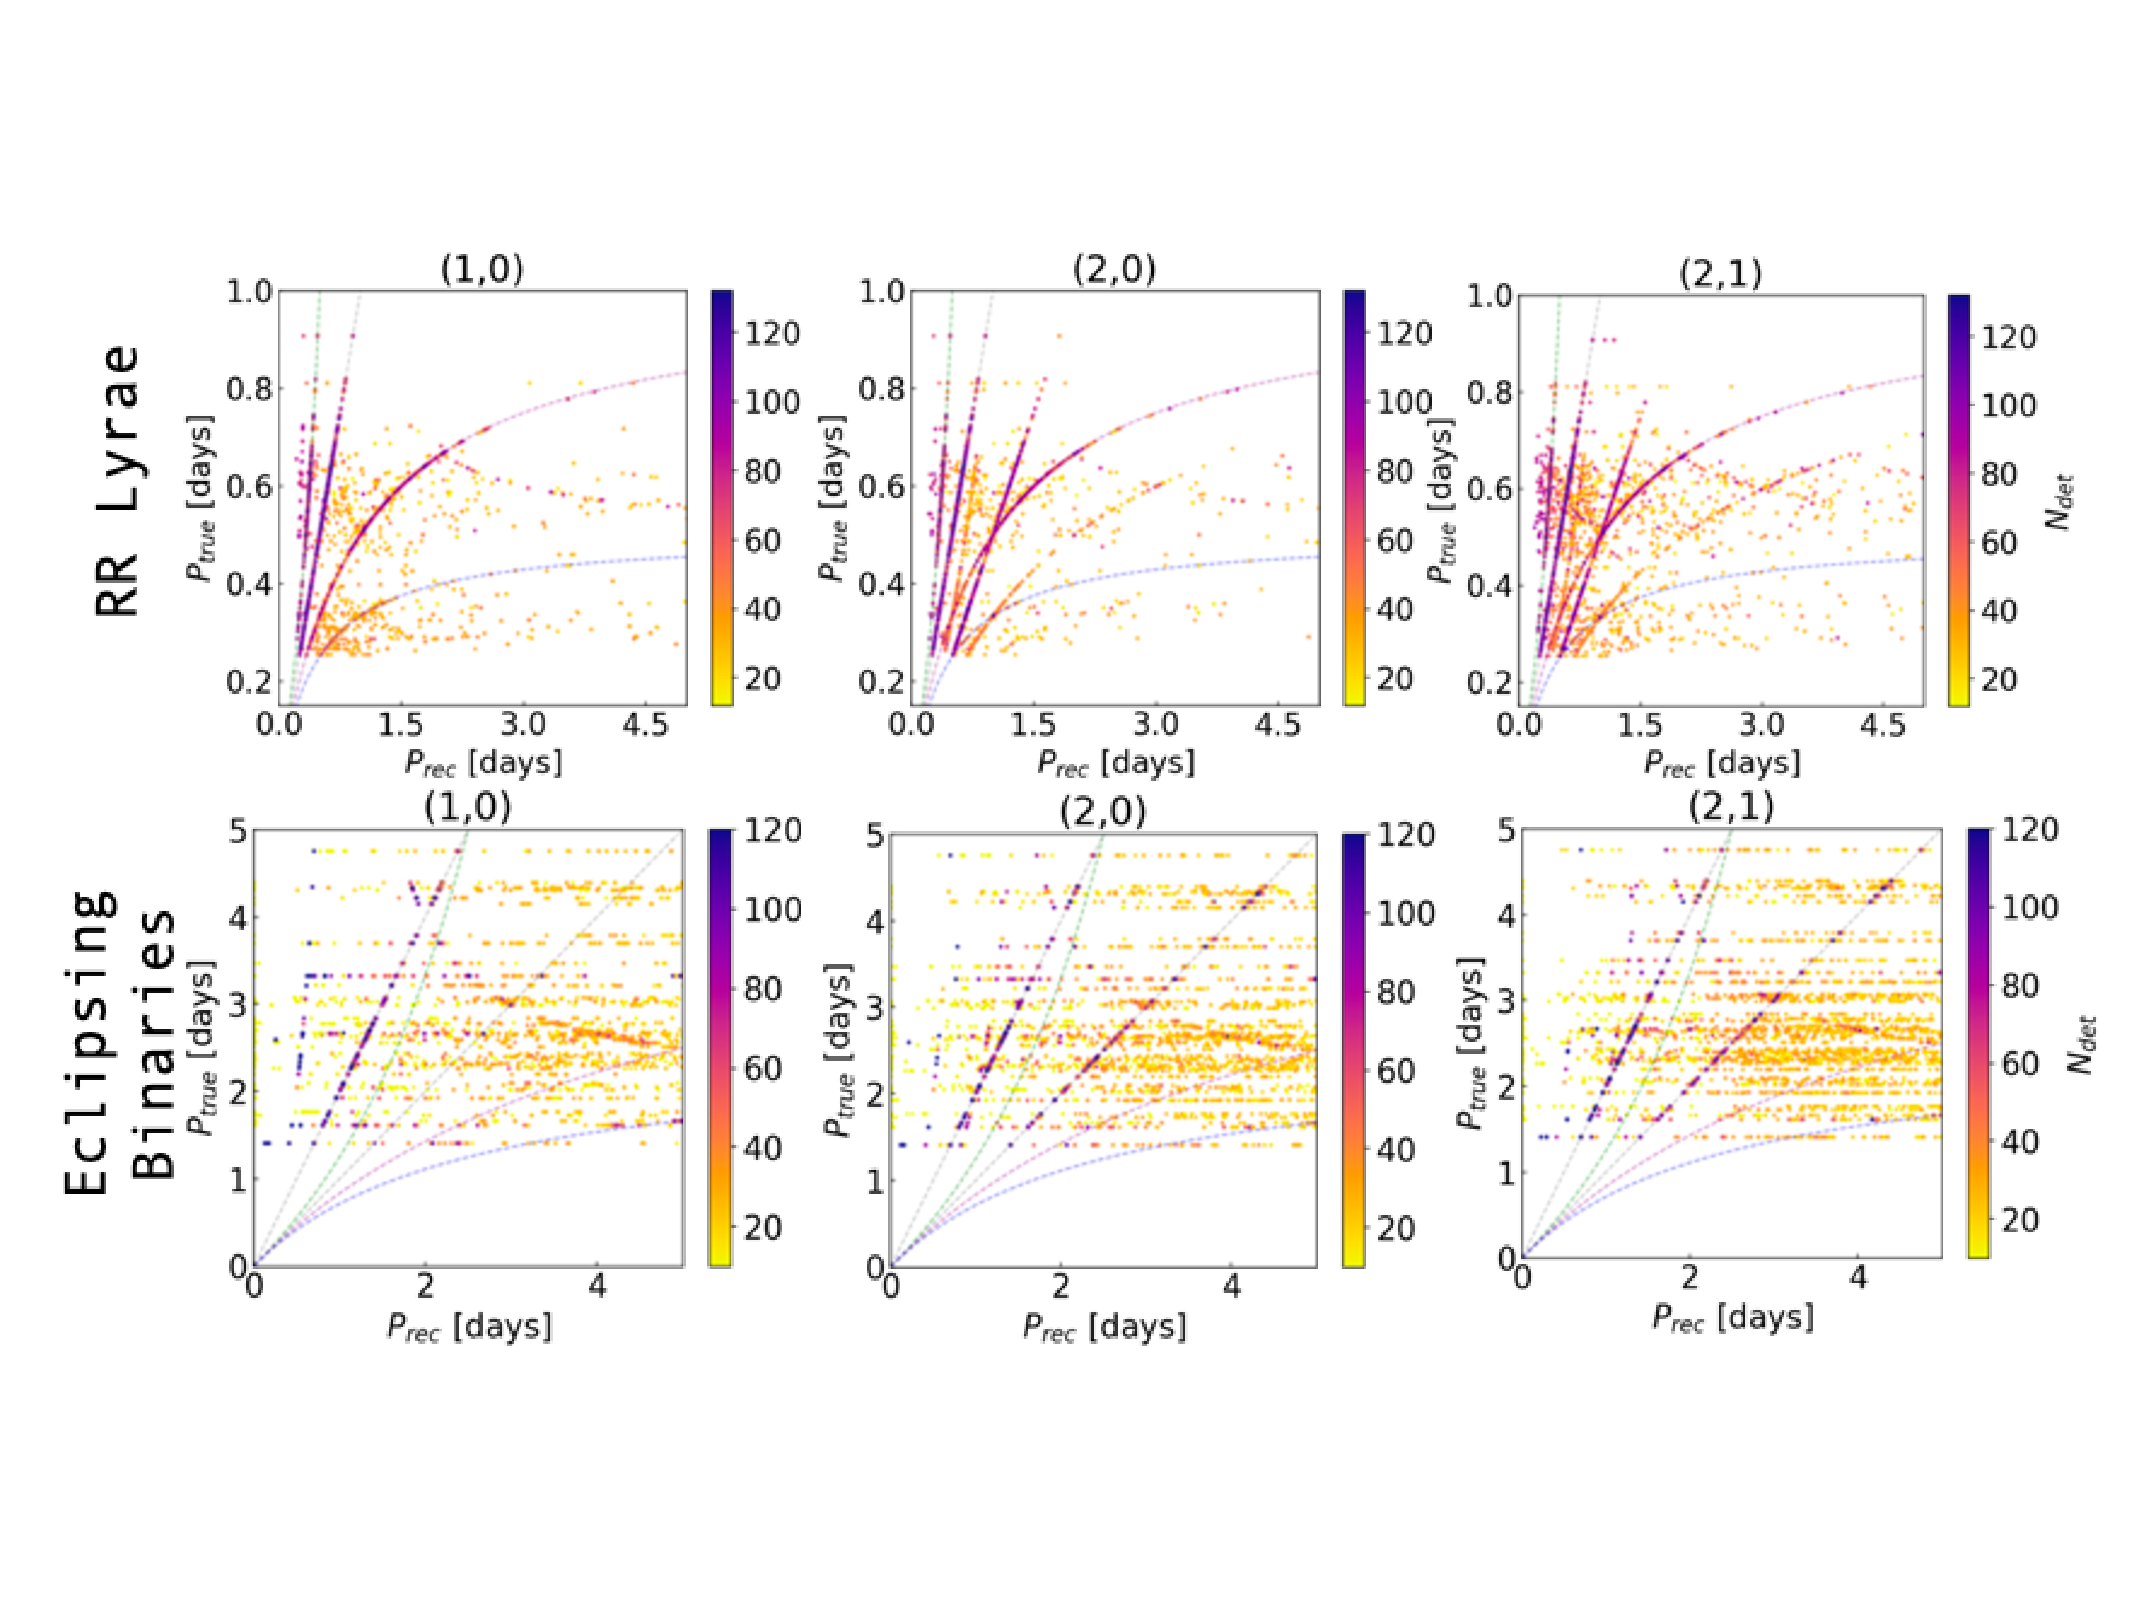
\includegraphics[width=0.9\textwidth]{figures/multi_lsp_rectest.pdf}
  \centering 
  \caption{Multi-band injection-recovery test for 5000 RR Lyrae (top row) and eclipsing binaries (bottom row). Each column title includes the number of Fourier base and band terms used to compute the Lomb-Scargle periodogram. Additionally we color code each recovered period by the number of detections. The overlaid curved lines represent the n=1 aliasing, while the straight lines represent the n=1,2 harmonics.}
  \label{fig:comp}
\end{figure*}


\subsection{Peak Significance Metric}

% TODO
\begin{itemize}
\item Bootstraping results 
\item Bootstrap results correlation with Baluev approximation
\item Application to other survey data (i.e SDSS)
\end{itemize}


\section{Timing Analysis}

% TODO
\begin{itemize}
\item Run time as a function of Fourier components (single band)
\item Run time as a function of Fourier components (multi-band)
\item Run time as a function of Nyquist frequency and oversampling factor
\end{itemize}


\appendix
% Include all the relevant bib files.
% https://lsst-texmf.lsst.io/lsstdoc.html#bibliographies
\section{References} \label{sec:bib}
\renewcommand{\refname}{} % Suppress default Bibliography section
\bibliography{local,lsst,lsst-dm,refs_ads,refs,books}

% Make sure lsst-texmf/bin/generateAcronyms.py is in your path
\section{Acronyms} \label{sec:acronyms}
\addtocounter{table}{-1}
\begin{longtable}{p{0.145\textwidth}p{0.8\textwidth}}\hline
\textbf{Acronym} & \textbf{Description}  \\\hline

AGN & active galactic nuclei \\\hline
CCD & Charge-Coupled Device \\\hline
DC2 & Data Challenge 2 (DESC) \\\hline
DIA & Difference Image Analysis \\\hline
DM & Data Management \\\hline
DMTN & DM Technical Note \\\hline
EB & ExaByte \\\hline
HR & Human Resources \\\hline
LSST & Legacy Survey of Space and Time (formerly Large Synoptic Survey Telescope) \\\hline
SDSS & Sloan Digital Sky Survey \\\hline
\end{longtable}

% If you want glossary uncomment below -- comment out the two lines above
%\printglossaries





\end{document}
